

%{\setbeamercolor{background canvas}{bg=tumbluedark}
%	\begin{frame}[plain]
%	
%	\begin{center}
%		\Huge\color{tumwhite}
%		Do cloudy observations have influence on the prediction?
%	\end{center}\color{white}
%	
%\end{frame}
%}
%
%{\setbeamercolor{background canvas}{bg=tumorange}
%\begin{frame}[plain]
%\vfill
%\begin{center}
%	\Huge\color{white}
%	Let's look at...
%\end{center}
%\vfill
%\end{frame}
%}
%
%{\setbeamercolor{background canvas}{bg=tumbluedark}
%	\begin{frame}[plain]
%	
%	\begin{center}
%		\vspace{3em}
%		\Huge\color{tumwhite}
%		...backpropagated gradients $\frac{\partial{\yhat}}{\partial\M{X}}$ from the prediction $\yhat$ to the input $\M{X}$
%		
%		\vspace{3em}
%		\raggedleft{\Large using a LSTM-RNN model}
%	\end{center}\color{white}
%	
%\end{frame}
%}

%{\setbeamercolor{background canvas}{bg=white}
%\begin{frame}[plain]
%
%\vspace{8em}
%\begin{center}
%	\Huge\color{tumbluedark}
%	with \textbf{gradients}
%\end{center}\color{white}
%
%\end{frame}
%}

\begin{frame}<presentation:4->
\only<1-3>{\frametitle{Usually we use gradients to adjust $\Mweight$...}}
\only<4->{\frametitle{Input feature importance analysis through gradient backpropagation}}

\centering
\begin{tikzpicture}
\node[font=\Huge](grad){
\only<1-3>{
$\frac{\partial \mathcal{L}(\V{y},f_\Mweight(\M{X}))}{\partial \Mweight}$
}
\only<4->{
\Huge$\frac{\partial \max(\yhat)}{\partial \M{X}}$
}
};

\node[above left=of grad, text width=10em](annotdx){
\only<2,3>{how do we have to change the network weights $\Mweight$...}
\only<4,5>{if we change the input $\M{X}$...} 
};
\node[below right=of grad, text width=10em](annotdy){
\only<3>{... to change (minimize) the loss $\mathcal{L}$?}
\only<5>{... how would the highest predicted score $\max(\yhat)$ change?}
};

\visible<2,3,4,5>{\draw[-stealth, shorten >= 1em, rounded corners] (annotdx) -| ($ (annotdx)!0.5!(grad) $) |- ($ (grad)+(-.5em, -1em) $);}
\visible<3,5>{\draw[-stealth, shorten >= 1em, rounded corners] (annotdy) -| ($ (annotdy)!0.5!(grad) $) |- ($ (grad)+(2.5em, 1em) $);}

\end{tikzpicture}
\end{frame}

\begin{frame}
\frametitle{Can be implemented in four lines}


%\Large $\frac{\partial \max(\yhat)}{\partial \M{X}}$ implementation

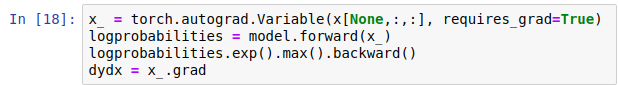
\includegraphics[width=\textwidth]{images/dydx_code}

\end{frame}


\begin{frame}
\frametitle{Gradients from $\max(\yhat)$ to \M{X}}

\vspace{-3em}
\begin{tikzpicture}

\def\root{images/rnn_examples/5}


\begin{groupplot}[
group style = {
group size = 1 by 2,
xlabels at=edge bottom,
xticklabels at=edge bottom,
vertical sep=0pt,
},
width=\textwidth,
%		hide axis,
enlargelimits=.1,
height=4cm,
xlabel=observation time $t$,
legend style={at={(1,1.8)},line width=2pt, draw opacity=1},
legend columns=4,
%ymin=-.2, ymax=.2,
%no marks,
]
\nextgroupplot[draw opacity=.8, smooth=0.01, ylabel=$\M{X}$]

\addplot[b2color, mark=*,mark size=.5pt] table [x=t, y=B2, col sep=comma] {\root/x.csv};
\addplot[b3color, mark=*,mark size=.5pt] table [x=t, y=B3, col sep=comma] {\root/x.csv};
\addplot[b4color, mark=*,mark size=.5pt] table [x=t, y=B4, col sep=comma] {\root/x.csv};

\addplot[b5color, mark=*,mark size=.5pt] table [x=t, y=B5, col sep=comma] {\root/x.csv};
\addplot[b6color, mark=*,mark size=.5pt] table [x=t, y=B6, col sep=comma] {\root/x.csv};
\addplot[b7color, mark=*,mark size=.5pt] table [x=t, y=B7, col sep=comma] {\root/x.csv};
\addplot[b8color, mark=*,mark size=.5pt] table [x=t, y=B8, col sep=comma] {\root/x.csv};
\addplot[b8Acolor, mark=*,mark size=.5pt] table [x=t, y=B8A, col sep=comma] {\root/x.csv};

\addplot[b11color, mark=*,mark size=.5pt] table [x=t, y=B11, col sep=comma] {\root/x.csv};
\addplot[b12color, mark=*,mark size=.5pt] table [x=t, y=B12, col sep=comma] {\root/x.csv};


\legend{B02 (blue),B03 (green),B04 (red),B05,B06,B07,B08,B8A,B11,B12}

\node[anchor=west](annotclouds) at (axis cs:-3,1){clouds};
\draw[-stealth](annotclouds) -- (axis cs:3,.75);

\node[anchor=west](annotnoclouds) at (axis cs:30,1){no clouds};
\draw[-stealth](annotnoclouds) -- (axis cs:33,.35);


\nextgroupplot[draw opacity=.8, smooth=0.01, ylabel=$\frac{\partial \max(\yhat)}{\partial \V{X}}$, ymin=-3, ymax=3]
\addplot[b11color, mark=*,mark size=.5pt] table [x=t, y=B11, col sep=comma, forget plot] {\root/dydx.csv};
\addplot[b12color, mark=*,mark size=.5pt] table [x=t, y=B12, col sep=comma] {\root/dydx.csv};

\addplot[b5color, mark=*,mark size=.5pt] table [x=t, y=B5, col sep=comma, forget plot] {\root/dydx.csv};
\addplot[b6color, mark=*,mark size=.5pt] table [x=t, y=B6, col sep=comma, forget plot] {\root/dydx.csv};
\addplot[b7color, mark=*,mark size=.5pt] table [x=t, y=B7, col sep=comma, forget plot] {\root/dydx.csv};
\addplot[b8color, mark=*,mark size=.5pt] table [x=t, y=B8, col sep=comma, forget plot] {\root/dydx.csv};
\addplot[b8Acolor, mark=*,mark size=.5pt] table [x=t, y=B8A, col sep=comma] {\root/dydx.csv};

\addplot[b2color, mark=*,mark size=.5pt] table [x=t, y=B2, col sep=comma, forget plot] {\root/dydx.csv};
\addplot[b3color, mark=*,mark size=.5pt] table [x=t, y=B3, col sep=comma, forget plot] {\root/dydx.csv};
\addplot[b4color, mark=*,mark size=.5pt] table [x=t, y=B4, col sep=comma] {\root/dydx.csv};

\node[anchor=west](annotcloudsgrad) at (axis cs:-3,2.5){no gradients};
\draw[-stealth](annotcloudsgrad) -- (axis cs:3,0);

\node[anchor=west](annotnoclouds) at (axis cs:35,2.5){gradients};
\draw[-stealth](annotnoclouds) -- (axis cs:33,1.8);

\end{groupplot}
\end{tikzpicture}
\end{frame}


\begin{frame}<presentation:0>
\begin{tikzpicture}

\frametitle{Gradients from $\max(\yhat)$ to \M{X}}
\framesubtitle{Example 2}

\def\root{images/rnn_examples/6}


\begin{groupplot}[
group style = {
group size = 1 by 2,
xlabels at=edge bottom,
xticklabels at=edge bottom,
vertical sep=0pt,
},
width=\textwidth,
%		hide axis,
enlargelimits=.1,
height=4cm,
xlabel=observation time $t$,
%ymin=-.2, ymax=.2,
%no marks,
]
\nextgroupplot[draw opacity=.8, smooth=0.01, ylabel=$\M{X}$]
\addplot[b11color, mark=*,mark size=.5pt] table [x=t, y=B11, col sep=comma, forget plot] {\root/x.csv};
\addplot[b12color, mark=*,mark size=.5pt] table [x=t, y=B12, col sep=comma] {\root/x.csv};

\addplot[b5color, mark=*,mark size=.5pt] table [x=t, y=B5, col sep=comma, forget plot] {\root/x.csv};
\addplot[b6color, mark=*,mark size=.5pt] table [x=t, y=B6, col sep=comma, forget plot] {\root/x.csv};
\addplot[b7color, mark=*,mark size=.5pt] table [x=t, y=B7, col sep=comma, forget plot] {\root/x.csv};
\addplot[b8color, mark=*,mark size=.5pt] table [x=t, y=B8, col sep=comma, forget plot] {\root/x.csv};
\addplot[b8Acolor, mark=*,mark size=.5pt] table [x=t, y=B8A, col sep=comma] {\root/x.csv};

\addplot[b2color, mark=*,mark size=.5pt] table [x=t, y=B2, col sep=comma, forget plot] {\root/x.csv};
\addplot[b3color, mark=*,mark size=.5pt] table [x=t, y=B3, col sep=comma, forget plot] {\root/x.csv};
\addplot[b4color, mark=*,mark size=.5pt] table [x=t, y=B4, col sep=comma] {\root/x.csv};

\nextgroupplot[draw opacity=.8, smooth=0.01, ylabel=$\frac{\partial \max(\yhat)}{\partial \V{X}}$]
\addplot[b11color, mark=*,mark size=.5pt] table [x=t, y=B11, col sep=comma, forget plot] {\root/dydx.csv};
\addplot[b12color, mark=*,mark size=.5pt] table [x=t, y=B12, col sep=comma] {\root/dydx.csv};

\addplot[b5color, mark=*,mark size=.5pt] table [x=t, y=B5, col sep=comma, forget plot] {\root/dydx.csv};
\addplot[b6color, mark=*,mark size=.5pt] table [x=t, y=B6, col sep=comma, forget plot] {\root/dydx.csv};
\addplot[b7color, mark=*,mark size=.5pt] table [x=t, y=B7, col sep=comma, forget plot] {\root/dydx.csv};
\addplot[b8color, mark=*,mark size=.5pt] table [x=t, y=B8, col sep=comma, forget plot] {\root/dydx.csv};
\addplot[b8Acolor, mark=*,mark size=.5pt] table [x=t, y=B8A, col sep=comma] {\root/dydx.csv};

\addplot[b2color, mark=*,mark size=.5pt] table [x=t, y=B2, col sep=comma, forget plot] {\root/dydx.csv};
\addplot[b3color, mark=*,mark size=.5pt] table [x=t, y=B3, col sep=comma, forget plot] {\root/dydx.csv};
\addplot[b4color, mark=*,mark size=.5pt] table [x=t, y=B4, col sep=comma] {\root/dydx.csv};

\end{groupplot}
\end{tikzpicture}
\end{frame}


\begin{frame}<presentation:0>
\begin{tikzpicture}

\frametitle{Gradients from $\max(\yhat)$ to \M{X}}
\framesubtitle{Example 3}

\def\root{images/rnn_examples/7}


\begin{groupplot}[
group style = {
group size = 1 by 2,
xlabels at=edge bottom,
xticklabels at=edge bottom,
vertical sep=0pt,
},
width=\textwidth,
%		hide axis,
enlargelimits=.1,
height=4cm,
xlabel=observation time $t$,
%ymin=-.2, ymax=.2,
%no marks,
]
\nextgroupplot[draw opacity=.8, smooth=0.01, ylabel=$\M{X}$]
\addplot[b11color, mark=*,mark size=.5pt] table [x=t, y=B11, col sep=comma, forget plot] {\root/x.csv};
\addplot[b12color, mark=*,mark size=.5pt] table [x=t, y=B12, col sep=comma] {\root/x.csv};

\addplot[b5color, mark=*,mark size=.5pt] table [x=t, y=B5, col sep=comma, forget plot] {\root/x.csv};
\addplot[b6color, mark=*,mark size=.5pt] table [x=t, y=B6, col sep=comma, forget plot] {\root/x.csv};
\addplot[b7color, mark=*,mark size=.5pt] table [x=t, y=B7, col sep=comma, forget plot] {\root/x.csv};
\addplot[b8color, mark=*,mark size=.5pt] table [x=t, y=B8, col sep=comma, forget plot] {\root/x.csv};
\addplot[b8Acolor, mark=*,mark size=.5pt] table [x=t, y=B8A, col sep=comma] {\root/x.csv};

\addplot[b2color, mark=*,mark size=.5pt] table [x=t, y=B2, col sep=comma, forget plot] {\root/x.csv};
\addplot[b3color, mark=*,mark size=.5pt] table [x=t, y=B3, col sep=comma, forget plot] {\root/x.csv};
\addplot[b4color, mark=*,mark size=.5pt] table [x=t, y=B4, col sep=comma] {\root/x.csv};

\nextgroupplot[draw opacity=.8, smooth=0.01, ylabel=$\frac{\partial \max(\yhat)}{\partial \V{X}}$]
\addplot[b11color, mark=*,mark size=.5pt] table [x=t, y=B11, col sep=comma, forget plot] {\root/dydx.csv};
\addplot[b12color, mark=*,mark size=.5pt] table [x=t, y=B12, col sep=comma] {\root/dydx.csv};

\addplot[b5color, mark=*,mark size=.5pt] table [x=t, y=B5, col sep=comma, forget plot] {\root/dydx.csv};
\addplot[b6color, mark=*,mark size=.5pt] table [x=t, y=B6, col sep=comma, forget plot] {\root/dydx.csv};
\addplot[b7color, mark=*,mark size=.5pt] table [x=t, y=B7, col sep=comma, forget plot] {\root/dydx.csv};
\addplot[b8color, mark=*,mark size=.5pt] table [x=t, y=B8, col sep=comma, forget plot] {\root/dydx.csv};
\addplot[b8Acolor, mark=*,mark size=.5pt] table [x=t, y=B8A, col sep=comma] {\root/dydx.csv};

\addplot[b2color, mark=*,mark size=.5pt] table [x=t, y=B2, col sep=comma, forget plot] {\root/dydx.csv};
\addplot[b3color, mark=*,mark size=.5pt] table [x=t, y=B3, col sep=comma, forget plot] {\root/dydx.csv};
\addplot[b4color, mark=*,mark size=.5pt] table [x=t, y=B4, col sep=comma] {\root/dydx.csv};

\end{groupplot}
\end{tikzpicture}
\end{frame}